% AUTO-GENERATED by writeup/make_rehaul_economics.py -- do not edit; re-run the script.
\begin{figure}[tbp]
\centering
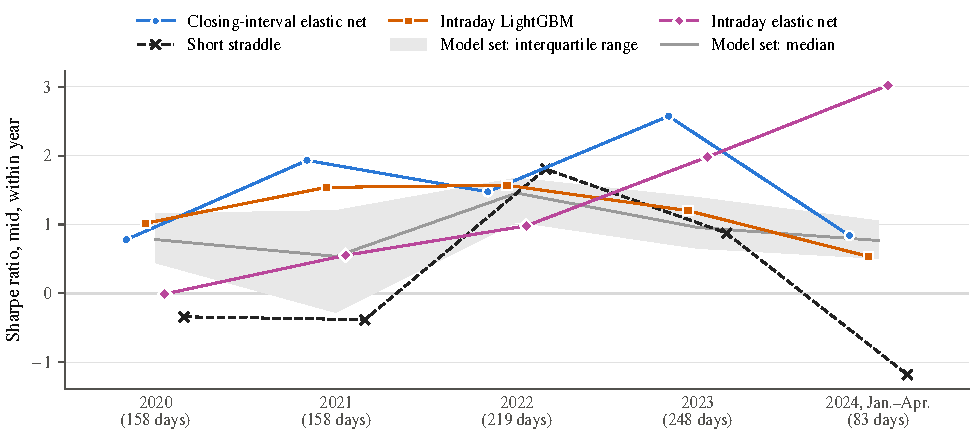
\includegraphics[width=\linewidth]{figures/rehaul_econ_byyear.pdf}
\caption{Sharpe ratio by calendar year at mid, $q_t = \sign(\hat\sigma^2_t - \mathrm{IV}^2_t)$, for the forecasts of
Figure~\ref{fig:rh_econ_cumpnl} and the short-straddle benchmark (2020 to 2024: $-0.34$, $-0.38$, $1.81$, $0.88$, $-1.18$); 2024 runs from
January to April. Each year's ratio is $\SR_y$ of Section~\ref{sec:rh_econ_measures}, scaled by the square root of that year's number of option days. Grey: the interquartile range
and median of the 112 forecasts of the model set (median $0.78$, $0.54$, $1.46$, $0.96$, $0.77$).}
\label{fig:rh_econ_byyear}
\end{figure}
